\documentclass{beamer}
\DeclareFontShape{OT1}{cmss}{b}{n}{<->ssub * cmss/bx/n}{} 
\usetheme{default}
\usepackage{amsmath}
\usepackage{amsfonts}
\usepackage{mathbbol}
\usepackage{xcolor} % before tikz or tkz-euclide if necessary
\usepackage{tkz-euclide} % no need to load TikZ
\usepackage{multirow}
\usepackage{lmodern}
\usepackage{bm}
\usepackage{csquotes}
\usepackage{graphicx}

\titlegraphic{
\includegraphics[width=2cm]{../../Figures/UAMS_RGB.png}
}


\title{Adjusting the $p$-values' role \\  in Biomedical Research}
\author{Horacio G\'omez-Acevedo\\ Department of Biomedical Informatics\\
University of Arkansas for Medical Sciences}
\begin{document}
	\begin{frame}[plain]
		\maketitle
	\end{frame}
	\begin{frame}{What is a $p$-value?}
		
		Ingredients:
\begin{itemize}
	\item Data (random sample)
	\item Statistic (a special type of function)
	\item A value (called the level of significance)
	\item A (null) hypothesis $H_0$	
\end{itemize}		

\begin{definition}
	The $p$-value is the observed tail probability of a statistic being at least as extreme as the particular observed value when $H_0$ is true.
\end{definition}		
		
		
	

		
	\end{frame}

\begin{frame}{What is a $p$-value?(cont)}
	Analog in Criminal trials
	
	If the defendant is innocent, what is the chance that we would observe such extreme criminal evidence?

	
\href{https://newonlinecourses.science.psu.edu/statprogram/reviews/statistical-concepts/hypothesis-testing/p-value-approach}{Source}

\end{frame}
	



\begin{frame}{The problem of statistical significance}
	
In the mind of hypothetical researcher:

\begin{displayquote}
	I used one-way ANOVA to differentiate the femur BMD between wildtype and two genotypes and I got $p$-value $<0.049$, thus the results are \textbf{statistically significant}"  ... (champagne is in order!!) 
\end{displayquote}

\begin{displayquote}
However, I checked body weight of those genotypes at 6 months and I got $p$-value $= 0.051$. I cannot reproduce what I saw last time!... (throw the experiment away and never talk about it!!)
\end{displayquote}

\end{frame}

\begin{frame}{What is the problem with that?}
The $p$-value and the threshold (typically $0.05$) should NEVER (EVER) used as a test for no association or no difference. 

In other words 

\begin{displayquote}
\textbf{STOP CATEGORIZING BASED ONLY ON $p$-VALUES}
\end{displayquote}

The phrase \textbf{statistically significant} should be discontinued because it supports false assumptions of difference or lack thereof. 
\end{frame}

\begin{frame}{It is not a new problem!}
It has been on statistical circles (and research) for more than a decade. 
The American Statistical Association had an special issue in 2018 about this very topic on the journal \textbf{The American Statistician}.

\begin{displayquote}
When I see articles with lots of significance test, I say that the statisticians are p-ing on the research\\
Herman Friedman
\end{displayquote}

\end{frame}

\begin{frame}{What does the ASA say?}

In 2016, the American Statistical Association released an statement about this:

- $p$-values can indicate how incompatible the data are with a specified statistical model.

- $p$-values do not measure the probability that the studied hypothesis is true, or the probability that the data were produced by random chance alone.

\end{frame}

\begin{frame}{What does the ASA say? (cont)}
	
	\begin{itemize}
		\item Scientific conclusions and business or policy decisions should not be based only on whether a $p$-values passes a specific threshold.
		\item Proper inference requires full reporting and transparency.
		\item A $p$-value, or statistical significance, does not measure the size of an effect or the importance of a result.
		\item  By itself, a $p$-value does not provide a good measure of evidence regarding a model or hypothesis.
	\end{itemize}

\end{frame}

\begin{frame}{Some important points}

\begin{itemize}
	\item No $p$-value can reveal the plausibility, presence,
	truth, or importance of an association or effect. 
	\item  A label of statistical significance does not mean or imply that an
	association or effect is highly probable, real, true, or important.
	\item Nor does a label of statistical nonsignificance lead to the association
	or effect being improbable, absent, false, or unimportant
\end{itemize}

\begin{displayquote}
	Significant" and "not significant" is not itself statistically significant.\\
	
	Gelman and Stern (2006)

\end{displayquote}


\end{frame}

\begin{frame}{We are affecting the scientific process}

Jessica Utts (ASA former president)

"Over time it appears that $p$-value become a gatekeeper for whether work is publishable ... this apparent editorial bias leads to the *file-drawer effect* in which research with statistically significant outcomes are more likely to get published, while other work that might well be just as important scientifically is never seen print."

The end result will bias the very research endeavour that we are involved in..

\end{frame}

\begin{frame}{Sort of good news?}

Wasserstein et al (2018) point out that 

\begin{itemize}
	\item There is not a solution that majestically replaces the outsized role that statistical significance has come to play.
	\item The statistical community has not yet converged on a simple paradigm for the use of statistical inference in scientific research.
\end{itemize}

\end{frame}

\begin{frame}{Sort of good news?}

Recommendations, use the \textbf{ATOM} methodology

\begin{itemize}
	\item  \textbf{A}ccept uncertainty. 
	\item Be \textbf{T}houghtful, 
	\item  \textbf{O}pen, and 
	\item \textbf{M}odest
\end{itemize}


\end{frame}

\begin{frame}{Accept uncertainty}
\begin{itemize}
	\item With every point estimate we add a measure of its uncertainty (e.g., standard error, interval estimate).
	\item Report and interpret point and interval estimate. 
	\item  Start thinking of confidence intervals as "compatibility intervals" which use $p$-values to show the effect sizes that are most compatible with the data under the given model.
\end{itemize}

\end{frame}

\begin{frame}{Be Thoughtful}
Answer some (or all) of these questions
\begin{itemize}
	\item What are the practical implications of the estimate?
	\item How precise is the estimate?
	\item Is the model correctly specified?
	\item Are the modeling assumptions understood?
	\item Are the assumptions valid?
	\item Do the key results hold up when other modeling choices are made?
\end{itemize}

\end{frame}

\begin{frame}{Be Thoughtful (cont.)}
\begin{figure}[!htb]
	\centering
	\begin{minipage}{.5\textwidth}
		\centering
		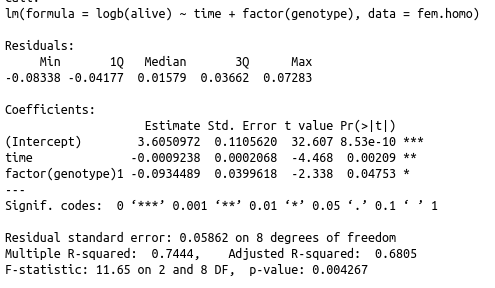
\includegraphics[width=1.2\linewidth]{../../Figures/females_date_rates_stats.png}
	%	\caption{$dt=0.1$}
%		\label{fig:prob1_6_2}
	\end{minipage}%
	\begin{minipage}{0.5\textwidth}
		\centering
		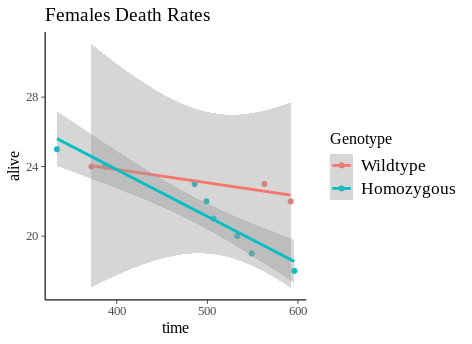
\includegraphics[width=1.2\linewidth]{../../Figures/females_death_rates.png}
	%	\caption{$dt =$}
	%	\label{fig:prob1_6_1}
	\end{minipage}
\end{figure}

\end{frame}


\begin{frame}{Be Thoughtful (and fancy)}
There are multiple approaches to complement the $p$-values.

\begin{itemize}
	\item Greenland et al (2019) suggest the use $s$-values (Shannon information $s=-\log_2 (p)$) that moves users away from probability misinterpretation.
	\item Second generation $p$-values (SGPV) from Blume et al. They claim that it lowers false discovery rates and more likely it would be reproducible in future studies.
\end{itemize}

\end{frame}

\begin{frame}{Be Open}
	
\begin{itemize}
	\item  Public pre-registration of methods
	\item Transparency
	\item Completeness in reporting
\end{itemize}	
Personal decision making is part of statistical data analysis, but it should be openly disclosed, so other researchers can execute maninful alternative analyses.
\end{frame}

\begin{frame}{Be Modest}

\begin{itemize}
	\item There is not a "true statistical model" underlying every problem.
	\item $p$-values, confidence intervals and other statistical measures are all uncertain.
	\item The nexus of opennes and modesty is to report everything while at the same time not concluding anything from a single study with unwarranted certainty. 
	\item Encourage others to reproduce your work. 
\end{itemize}
	
\end{frame}

\begin{frame}{Change is slow}
We can start with replacing

\begin{itemize}
	\item $p$-values with an equality (not inequality)
	\item  if you obtain $p=0.03$" avoid using the phrase **statistically significant**
	\item  if you obtain $p=0.25$" avoid using the phrase **was not statistically significant** just report the value.
	\item  compare groups and studies directly by showing $p$-values and interval estimates for their differences, for instance $p$-values and confidence interval for the different for sex-specific associations. 
	\item never use the phrase \textbf{approaching to significance} 
\end{itemize}

\end{frame}

\begin{frame}{Book Example}
Sixty-six women with osteoporosis were alternately assigned to one of three treatment groups: Group 1 ($n=22$), group 2 ($n=22$), and controls ($n=22$). After 6 weeks, the change in BMD from baseline was measured. Analysis with one-way ANOVA ~~indicated a statistically significant difference between the groups $(F_{2,63}=61.07;P<0.0001)$~~ had a $p=1\times 10^{-4}$ ($F_{2,63}=61.07$).
\end{frame}


\begin{frame}{Book Example (cont.)}
Further analysis with Tukey's pair-wise comparison procedure to control for multiple testing revealed that ~~the mean change (\( \pm \)SD) of group 2 (1.6 $g/cm^2 \pm 0.2$) was significantly greater than of group 1 (1.1 $g/cm^2\pm 0.2$) and that of the controls (1.0 $g/cm^2 \pm 0.2$) with an overall alpha level of $0.05$.~~ group 2 has a higher mean (1.6 $g/cm^2$), than group 1 (1.1 $g/cm^2$) and controls (1.0$g/cm^2$). The 90\% confidence intervals for groups 2, 1 and controls are $(1.5,1.8)$, $(1.05,1.15)$, and $(0.85,1.15)$, respectively.  

From Land and Secic: How to report statistics in medicine (2005)
	
\end{frame}

\begin{frame}{Final thoughts}
\begin{itemize}
	\item Abuse of (click and play) statistical software 
	\item It obscures reproducibility
	\item Some of the warnings of modeling are hidden
	\item New methodologies are not implemented.
\end{itemize}	
	
	
\end{frame}


\begin{frame}{When you see a $p$-value}
	Recall ATOM (ant) 

\begin{figure}[!htb]
		\centering
		
\includegraphics[width=0.5\linewidth]{../../Figures/atom_ant.jpg}
		%	\caption{$dt=0.1$}
		%		\label{fig:prob1_6_2}
\end{figure}
\end{frame}




\end{document}